\documentclass{article}

    % Input language encoding
    %\usepackage[utf8]{inputenc}
   
    % Output languages
    %\usepackage[greek, english]{babel}
    % \usepackage{alphabeta}
    
    % Fonts
    %\usepackage[T1,LGR]{fontenc}
    \usepackage{lmodern}

    % Images
    \usepackage{graphicx}
    \usepackage{float}
    \usepackage{caption}
    \usepackage{subcaption}

    % Math
    \usepackage{amsmath}

    % Paragraph Formatting
    \usepackage{parskip}

    % Code
    \usepackage{listings}

        

    \DeclareMathSizes{10}{10}{10}{10}
    \setlength{\parindent}{0cm}

    \title{Excercise 1.2-3}

\begin{document}

\pagenumbering{gobble}
\date{}
\author{}

\maketitle

We will be using the same technique as before with excercise 1.2-2, in order to visually determine the number, who is going to be interger.

In this case, we need to figure out when $ 100*n^{2} > 2^{n} $.

By plotting it in Matlab, we have the Figure \ref{fig:plot1}:

\begin{figure}
    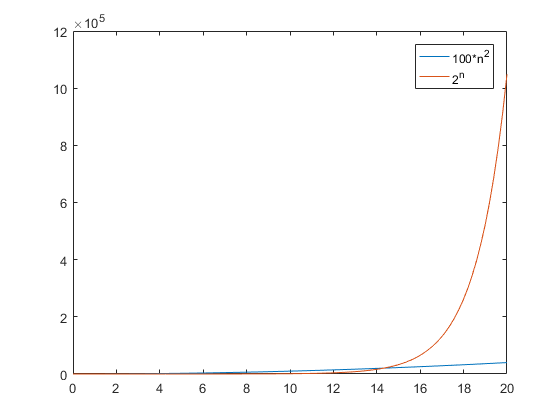
\includegraphics[width=10cm]{images/1-2-3.png}
    \centering
    \caption{Our plot}
    \label{fig:plot1}
\end{figure}

The Matlab code we used is the following:

\begin{lstlisting}[language=Matlab]
x = linspace(0, 20);
y1 = 100*x.^2;
y2 = 2.^x;
figure();
plot(x,y1,x,y2);
legend('100*n^2', '2^n');
\end{lstlisting}

As we see the period that $100n^{2}$ is slower than $2^{n}$ is until 14 inputs. After that (15 inputs onward) $2^{n}$ becomes considerably slower than $100*n^{2}$.

\end{document}